\documentclass[compress,red]{beamer}
\usepackage[utf8]{inputenc}
\usepackage{ucs}
\usepackage{amsmath}
\usepackage{amsfonts}
\usepackage{amssymb}
\usepackage[russian]{babel}
\usepackage{graphicx}
\usepackage{wrapfig}

\usepackage{tikz}
\usepackage{verbatim}

\usepackage{color}
\usepackage{xcolor}
\usepackage{listings}

\usepackage{caption}

\lstset{
language=ruby,
extendedchars=\true,
inputencoding=utf8x,
commentstyle=\itshape,
stringstyle=\bf,
belowcaptionskip=5pt }


\DeclareCaptionFont{white}{\color{white}}
\DeclareCaptionFormat{listing}{\colorbox{gray}{\parbox{\textwidth}{#1#2#3}}}
\captionsetup[lstlisting]{format=listing,labelfont=white,textfont=white}

\usetikzlibrary{calc,trees,positioning,arrows,chains,shapes.geometric,%
    decorations.pathreplacing,decorations.pathmorphing,shapes,%
    matrix,shapes.symbols}

\tikzset{
>=stealth',
  punktchain/.style={
    rectangle, 
    rounded corners, 
    % fill=black!10,
    draw=black, very thick,
    text width=10em, 
    minimum height=3em, 
    text centered, 
    on chain},
  line/.style={draw, thick, <-},
  element/.style={
    tape,
    top color=white,
    bottom color=blue!50!black!60!,
    minimum width=8em,
    draw=blue!40!black!90, very thick,
    text width=10em, 
    minimum height=1.5em, 
    text centered, 
    on chain},
  every join/.style={->, thick,shorten <=1pt},
  decoration={brace},
  tuborg/.style={decorate},
  tubnode/.style={midway, right=2pt},
}

\mode<presentation>

\usetheme{Warsaw}

\definecolor{Red}{rgb}{1,0,0}
\definecolor{Blue}{rgb}{0,0,1}
\definecolor{Green}{rgb}{0,1,0}
\definecolor{magenta}{rgb}{1,0,.6}
\definecolor{lightblue}{rgb}{0,.5,1}
\definecolor{lightpurple}{rgb}{.6,.4,1}
\definecolor{gold}{rgb}{.6,.5,0}
\definecolor{orange}{rgb}{1,0.4,0}
\definecolor{hotpink}{rgb}{1,0,0.5}
\definecolor{newcolor2}{rgb}{.5,.3,.5}
\definecolor{newcolor}{rgb}{0,.3,1}
\definecolor{newcolor3}{rgb}{1,0,.35}
\definecolor{darkgreen1}{rgb}{0, .35, 0}
\definecolor{darkgreen}{rgb}{0, .6, 0}
\definecolor{darkred}{rgb}{.75,0,0}

\xdefinecolor{olive}{cmyk}{0.64,0,0.95,0.4}
\xdefinecolor{purpleish}{cmyk}{0.75,0.75,0,0}

\useoutertheme[subsection=false]{smoothbars}

\title{Основы формальной и математической логик}

%\usecolortheme{dolphin}


\begin{document}
%%титульная страница
\maketitle
%% основные моменты

\section{Логика}

\subsection{КЭП}
\begin{frame}[fragile]
  \frametitle{Спасибо, КЭП}
  \centerline{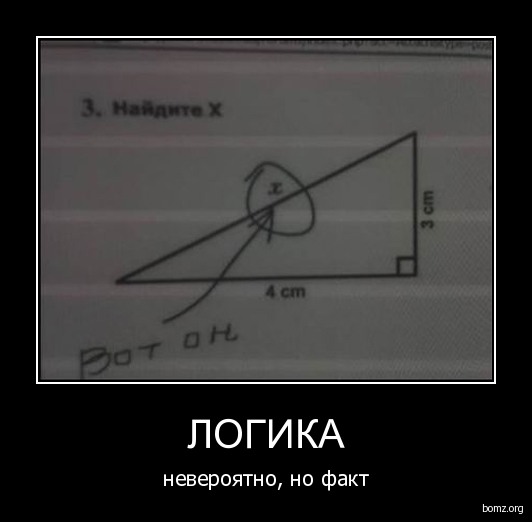
\includegraphics[width=0.7\textwidth]{images/logic.jpg}}
\end{frame}

\subsection{Логика}
\begin{frame}
  \frametitle{Логика}
  \begin{itemize}
    \item \emph{Логика} --- наука о законах и формах правильного рассуждения. 
    \item Главная задача логики --- прийти к выводу цепочкой последовательных рассуждений.
    \item Везде, в жизни, в образовании, в науке, в работе логика является \textbf{основным инструментом}.
  \end{itemize}
\end{frame}

\subsection{Логика в информатике}
\begin{frame}
  \frametitle{Логика в информатике}
  \begin{itemize}
    \item Составление алгоритмов и принципов работы устройств и программ.
    \item Программирование.
    \item Современные базы данных (к примеру, банковские операции).
    \item Вычисления и вычислительная математика.
    \item Искусственный интеллект и др.
  \end{itemize}
\end{frame}

\section{Формальная логика}
\subsection{Формальная логика}
\begin{frame}
  \begin{center}
    \Huge{Формальная логика}
  \end{center}
  \begin{center}
    \Large{конструирование цепочек последовательных истинных высказываний, следующих друг за другом.}
  \end{center}
\end{frame}

\subsection{Понятия формальной логики}
\begin{frame}[fragile]
  \frametitle{Неопределяемые понятия}
  \begin{itemize}
    \item Истина,
    \item ложь,
    \item высказывание (утверждение, суждение),
    \item равно (тождественно),
    \item и др.
  \end{itemize}
\end{frame}

\subsection{Законы формальной логики}
\begin{frame}
  \begin{center}
    \Huge{Законы формальной логики}
  \end{center}
\end{frame}

\subsection{Закон тождества}
\begin{frame}
  \begin{center}
    \Huge{Закон тождества}
  \end{center}
  \begin{center}
    \Large{Высказывание равно самому себе}
  \end{center}
\end{frame}

\subsection{Закон тождества 2}
\begin{frame}[fragile]
  \frametitle{Закон тождества}
  \begin{itemize}
    \item Закон утверждает, что высказывание должно быть ясным, точным, простым и определённым.
    \item Закон также требует определённости высказывания.
    \item Пример: \emph{Из-за рассеянности на турнирах шахматист неоднократно терял очки}.
    \item \emph{Гестаповцы ставили машину на попа. ``Бедный пастор,'' --- подумал
    Штирлиц.}
    \item \emph{Штирлиц бежал скачками. Скоро качки отстали.}
    \item \emph{Штирлиц знал наверняка. Но Наверняк не знал Штирлица.}
  \end{itemize}
\end{frame}

\subsection{Закон противоречия}
\begin{frame}
  \begin{center}
    \Huge{Закон противоречия}
  \end{center}
  \begin{center}
    \Large{Высказывание не может быть одновременно истинным и ложным.}
  \end{center}
\end{frame}

\subsection{Закон противоречия 2}
\begin{frame}[fragile]
  \frametitle{Закон противоречия}
  \begin{itemize}
    \item Закон противоречия запрещает одновременную истинность суждений, одно из которых что-то утверждает, а другое --- утверждает обратное.
    \item Закон, однако, не запрещает одновременную ложность обоих высказываний.
    \item \emph{Это не полезно, но и не вредно} --- оба утверждения (\emph{это полезно} и \emph{это вредно}) могут быть ложными одновременно.
  \end{itemize}
\end{frame}

\subsection{Закон исключённого третьего}
\begin{frame}
  \begin{center}
    \Huge{Закон исключённого третьего}
  \end{center}
  \begin{center}
    \Large{Высказывание либо истинно, либо ложно.}
  \end{center}
\end{frame}

\subsection{Закон исключённого третьего 2}
\begin{frame}[fragile]
  \frametitle{Закон исключённого третьего}
  \begin{itemize}
    \item Формальная логика этим законом требует, чтобы высказывание обязательно было либо истинным, либо ложным.
    \item При этом следует различать \emph{противоречивые} суждения и \emph{противоположные}.
    \item \emph{Вася --- дурак} и \emph{Вася --- умный} --- противоположные суждения.
    \item \emph{Вася --- дурак} и \emph{Вася --- не дурак} --- противоречивые суждения.
    \item Среди двух противоречивых утверждений одно обязано быть истинным, а одно --- ложным.
  \end{itemize}
\end{frame}

\section{Силлогизм}
\subsection{Силлогизм}
\begin{frame}
  \begin{center}
    \Huge{Силлогизм}
  \end{center}
\end{frame}

\subsection{Силлогизм}
\begin{frame}[fragile]
  \frametitle{Принцип тождества}
  \centerline{
\includegraphics[width=0.9\textwidth]{images/proof_or_fail.jpeg}}
\end{frame}

\subsection{Силлогизм}
\begin{frame}[fragile]
  \frametitle{Силлогизм}
  \begin{itemize}
    \item Силлогизм --- это традиционная логическая аргументация.
    \item 
      \begin{enumerate}
        \item Все бобры имеют хвост. 
        \item Вася --- бобёр. 
        \item Следовательно, Вася имеет хвост.
      \end{enumerate}
  \end{itemize}
\end{frame}

\subsection{Ошибки в силлогизмах 1}
\begin{frame}[fragile]
  \frametitle{Ошибки: нераспределённый средний термин}
  \begin{itemize}
    \item Все бобры имеют хвост.
    \item Все коты имеют хвост.
    \item Поэтому все коты --- бобры.
    \item \emph{Неверно, так как существуют коты необязательно должны быть бобрами, так как это нигде не утверждается.}
  \end{itemize}
\end{frame}

\subsection{Ошибки в силлогизмах 2}
\begin{frame}[fragile]
  \frametitle{Ошибки: аргумент из заблуждения}
  \begin{itemize}
    \item Все коты --- животные.
    \item Вася --- животное.
    \item Следовательно, Вася --- кот.
  \end{itemize}
\end{frame}

\subsection{Ошибки в силлогизмах 3}
\begin{frame}[fragile]
  \frametitle{Ошибки в причинно-следственной связи}
  \begin{itemize}
    \item
    \begin{enumerate}
      \item Если маленькие дети спят с включенным светом, то у них часто потом развивается близорукость.
      \item Следовательно, сон с включенным светом приводит к близорукости.
    \end{enumerate}
    \item Фактически, в первом утверждении не сказано ничего о том, именно включенный свет является причиной близорукости. Поэтому силлогизм неверен.
    \item На самом деле, близорукость передаётся по наследству, а родители, страдающие близорукостью, чаще оставляют свет включенным ночью.
  \end{itemize}
\end{frame}

\subsection{Фальшивая дилемма}
\begin{frame}[fragile]
  \frametitle{Фальшивая дилемма}
  \begin{itemize}
    \item
    \begin{enumerate}
      \item \emph{Ты за нас или за партию казнокрадов?}
    \end{enumerate}
    \item В данном случае не рассматривается вариант, когда человек может быть против обеих сторон.
    \item Аналогичный принцип: солгал в одном --- солгал во всём.
  \end{itemize}
\end{frame}

\subsection{Подтверждение консеквента}
\begin{frame}[fragile]
  \frametitle{Возможные причины}
  \begin{itemize}
    \item
    \begin{enumerate}
      \item Если я очень стараюсь, то добиваюсь успеха.
      \item Сегодня я добился успеха.
      \item Следовательно, я очень старался.
    \end{enumerate}
    \item В данном случае предполагается (и напрасно), что успех --- результат старания. При этом не указано, что за успех человек получил сегодня (мог ведь, к примеру, выиграть в лотерею).
  \end{itemize}
\end{frame}

\subsection{Отрицание антецедента и консеквента}
\begin{frame}[fragile]
  \frametitle{Отрицание}
  \begin{itemize}
    \item
    \begin{enumerate}
      \item Если я закончу университет, то я получу высокооплачиваемую работу.
      \item Поэтому если я не закончу университет, то я не получу высокооплачиваемую работу.
    \end{enumerate}
    \item Классическая ошибка в отрицании высказывания. Нигде не сказано, что \textbf{только} университет является единственной причиной хорошей работы.
  \end{itemize}
\end{frame}

\section{Операции в логике}
\subsection{Операции в логике}
\begin{frame}
  \begin{center}
    \Huge{Операции в логике}
  \end{center}
\end{frame}

\subsection{Операции в логике 2}
\begin{frame}[fragile]
  \frametitle{Операции в логике}
  \begin{itemize}
    \item В логике существуют операции, позволяющие связывать высказывания.
    \item Аналогия: сложение, умножение, отрицание.
    \item Логическое сложение называется \emph{дизъюнкцией} (логическое или), логическое умножение --- \emph{конъюнкцией} (логическое и) и отрицание (логическое не).
    \item Помимо этих операций есть и другие: \emph{импликация} --- ``следовательно'', эквиваленция --- ``равенство'' и другие.
  \end{itemize}
\end{frame}

\subsection{Операции в логике 3}
\begin{frame}[fragile]
  \frametitle{Примеры}
  \begin{itemize}
    \item Конъюнкция (и): Вася --- бобёр \textbf{и} Вася строит плотину.
    \item Дизъюнкция (или): Вася --- бобёр \textbf{или} Вася --- журавль. 
    \item Импликация (следовательно): Вася --- бобёр, следовательно, Вася имеет хвост.
    \item Эквиваленция (равносильно): Вася --- бобёр равносильно тому, что Вася имеет хвост.
  \end{itemize}
\end{frame}

\subsection{Отрицание}
\begin{frame}
  \begin{center}
    \Huge{Опасное отрицание}
  \end{center}
  \begin{center}
    \Large{Все бобры имеют хвост}
  \end{center}
\end{frame}

\subsection{Отрицание 2}
\begin{frame}
  \begin{center}
    \Huge{Отрицание}
  \end{center}
  \begin{center}
    \Large{\textbf{Не все бобры} имеют хвост}
  \end{center}
\end{frame}

\subsection{Операции 3}
\begin{frame}[fragile]
  \frametitle{Итоговые высказывания}
  \begin{itemize}
    \item Как и в случае с математикой, операции соединяют несколько высказываний в одно.
    \item В зависимости истинности составных частей и применяемой операции результат может быть разным.
    \item \emph{Вася --- мальчик или Вася --- девочка} --- истинное высказывание, ведь для \emph{или} достаточно истинности одной из частей.
    \item \emph{Вася --- мальчик и Вася --- девочка} --- ложное высказывание, так как для \emph{и} необходима истинность всех частей.
  \end{itemize}
\end{frame}

\subsection{Задание}
\begin{frame}[fragile]
  \frametitle{Задание}
  \begin{itemize}
    \item \textbf{Задание.} Рассмотрите все возможные варианты из двух высказывание (когда оба истинны, когда оба ложны и по одной истине/лжи) и их соединения с помощью конъюнкции и дизъюнкции. Каков будет результат в каждом из случаев? Приведите пример.
  \end{itemize}
\end{frame}

\subsection{Задание 2}
\begin{frame}[fragile]
  \frametitle{Парадокс брадобрея}
  \begin{itemize}
    \item В некотором городе все мужчины либо бреются сами, либо бреются у единственного в городе брадобрея. В этом же городе есть закон, согласно которому брадобрей бреет только тех людей, кто не бреется сам. Вопрос: бреет ли брадобрей сам себя?
  \end{itemize}
\end{frame}

\end{document}